\documentclass[12pt,letterpaper]{article}
\usepackage[latin1]{inputenc}
\usepackage{amsmath}
\usepackage{amsfonts}
\usepackage{amssymb}
\usepackage{amsthm}
\usepackage{enumerate}
\usepackage[margin=0.8in]{geometry}
\usepackage{graphicx}

\newtheorem{theorem}{Theorem}
\newtheorem{rem}[theorem]{Remark}
\newenvironment{remark}{\begin{rem}\rm}{\end{rem}}
\newtheorem{claim}[theorem]{Claim}
\newtheorem{lemma}[theorem]{Lemma}
\newtheorem{proposition}[theorem]{Proposition}
\newtheorem{corollary}[theorem]{Corollary}
\newtheorem{eg}[theorem]{Example}
\newenvironment{example}{\begin{eg}\rm}{\end{eg}}
\newtheorem{definition}[theorem]{Definition}

\newcommand{\C}{\mathbb{C}}
\newcommand{\dotp}{\boldsymbol{\cdot}}
\newcommand{\R}{\mathbb{R}}
\newcommand{\x}{\mathbf{x}}
\renewcommand{\r}{\mathbf{r}}
\newcommand{\F}{\mathbf{F}}
\renewcommand{\i}{\mathbf{i}}
\renewcommand{\j}{\mathbf{j}}
\renewcommand{\k}{\mathbf{k}}
\newcommand{\abs}[1]{\lvert#1\rvert}
\DeclareMathOperator{\Real}{Re}
\DeclareMathOperator{\Img}{Im}
\author{Sean Fitzpatrick}
\title{Path Independence and Conservative Vector Fields}

\begin{document}
\maketitle

Recall that in class we showed that for any gradient vector field $\F = \nabla f$, the line integral of $\F$ along a curve $C$ depends only on the endpoints of $C$. Our argument was as follows: let $C$ be a smooth oriented curve in $\R^n$ (for most purposes, $n=2$ or $n=3$, but this restriction is unnecessary), and let $\r:[a,b]\to \R^n$ be a parameterization of $C$, such that $\r(a) = P$ is the initial point of $C$, and $\r(b)=Q$ is the final point of $C$. By the definition of the line integral and the Fundamental Theorem of Calculus, we have
\[
 \int_C \nabla f\dotp d\r = \int_a^b \nabla f(\r(t))\dotp \r'(t) \,dt = \int_a^b \frac{d}{dt}(f(\r(t)))\,dt = f(\r(b))-f(\r(a)) = f(Q)-f(P).
\]
The answer therefore depends only on the endpoints. We call any vector field $\F$ with this property \textbf{conservative}. The above argument proves the following``
\begin{theorem}[Fundamental Theorem for Line Integrals]\label{T1}
 If $\F = \nabla f$ for some function $f$, then $\F$ is conservative, and $\int_C \F\dotp\, d\r = f(Q)-f(P)$ for any smooth oriented curve $C$ with initial point $P$ and final point $Q$.
\end{theorem}
The goal of this handout is to prove the converse:
\begin{theorem}\label{T2}
 Let $D$ be an open\footnote{An open subset of $\R^n$ is one that does not contain its boundary points; for example, the set $\{(x,y)\in
\R^2 | x^2+y^2<1\}$ consisting of all points inside the unit circle (the boundary of the set), but not the circle itself} connected\footnote{A connected subset of $\R^n$ is one that cannot be separated into two or more pieces, with ``gaps'' in between. For the purposes of this theorem, it's enough to know that any open, connected subset of $\R^n$ is \textbf{path-connected}, meaning that any two points in the set can be joined by a continuous curve.} If $\F$ is a continuous, conservative vector field on defined on $D$, then there exists a $C^1$ function $f:D\to\R$ such that $\F = \nabla f$.
\end{theorem}
\begin{proof}
 We prove the theorem by explicitly constructing the function $f$. (If we view Theorem \ref{T1} as the analogue of Part II of the Fundamental Theorem of Calculus, then this is the analogue of Part I.) Fix a point $\mathbf{a}=(a_1,a_2,\ldots, a_n)\in D$, and define a function $f:D\to\R$ by
\[
 f(x_1,x_2,\ldots, x_n) = \int_C \F\dotp \,d\r,
\]
where $C$ is any curve contained in $D$ with initial point $\mathbf{a}$ and final point $\mathbf{x}=(x_1,x_2,\ldots, x_n)$. (The assumption that $D$ is an open, connected set guarantees that such a curve $C$ exists.) Since $\F$ is conservative, the above integral depends only on $\mathbf{x}$, and not the curve $C$, so that $f$ is indeed a well-defined function. (That is, the value of $f(\mathbf{x})$ is uniquely determined by $\mathbf{x}$.)

To simplify notation, we'll take $n=3$, with $\F=P\i+Q\j+R\k$, and initial point $(a,b,c)$ and final point $(x,y,z)$ for the curve $C$. The general proof is similar.
We want to show that $\nabla f = \F$, so we begin by showing that $\dfrac{\partial f}{\partial x} = P$. Since $C$ can be any curve with initial point $(a,b,c)$ and final point $(x,y,z)$, we choose a curve of the form $C=C_1+C_2$, defined as follows:

First, choose a fixed value $x_0$ sufficiently close to $x$, such that the line segment from $(x_0,y,z)$ to $(x,y,z)$ lies entirely within $D$. We let $C_1$ be an arbitrary curve from $(a,b,c)$ to $(x_0,y,z)$, and we let $C_2$ be the line segment from $(x_0,y,z)$ to $(x,y,z)$. Thus,
\[
 \int_C\F\dotp\,d\r = \int_{C_1+C_2}\F\dotp\,d\r = \int_{C_1}\F\dotp\,d\r +\int_{C_2}\F\dotp\,d\r .
\]
The first integral does not depend on $x$, so we have
\[
 \frac{\partial}{\partial x}\int_C\F\dotp\,d\r = 0+\frac{\partial}{\partial x}\int_{C_2}\F\dotp\,d\r. 
\]
For the second integral, we parameterize $C_2$ using $r(t) = \langle t, y, z\rangle$, with $t\in [x_0,x]$. This gives us
\[
 \F\dotp\,d\r = P\,dx+Q\,dy+R\,dz  = P(t,y,z)\,dt,
\]
since $dt = dx$, and $dy=dz=0$ (we're holding $y$ and $z$ constant). We then have
\[
 \frac{\partial}{\partial x}\int_{C_2}\F\dotp\,d\r = \frac{\partial }{\partial x}\int_{x_0}^x P(t,y,z)\,dt = P(x,y,z),
\]
by the Fundamental Theorem of Calculus. The proofs that $f_y=Q$ and $f_z=R$ are similar.
\end{proof}
\begin{figure}
\begin{center}
 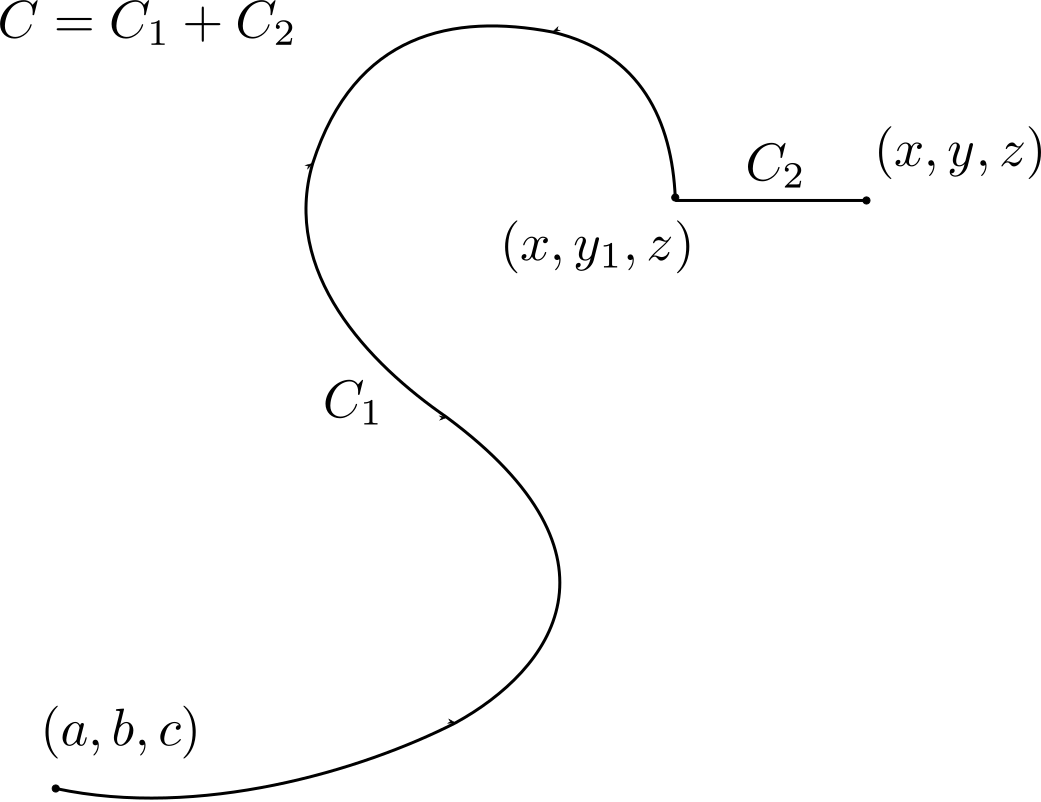
\includegraphics[width=0.6\textwidth]{conservative}
\end{center}
 \caption{The curve $C$ used to calculate $\dfrac{\partial f}{\partial y}$.}
\end{figure}


We also have the following result:
\begin{theorem}
 A vector field $\F$ is conservative if and only if $\int_C\F\dotp\,d\r$ for every \textbf{closed} curve $C$.
\end{theorem}

To see that this result is true, notice that by Theorem \ref{T2}, if $\F$ is conservative (that is, if $\int_C \F\dotp \,d\r$ is independent of path), then $\F=\nabla f$ for some function $f$, so if $C$ is a closed curve parameterized by $\r(t)$, $t\in [a,b]$, we have $\r(a)=\r(b)$, and thus
\[
 \int_C\F\dotp\,d\r = \int_C\nabla f\dotp \,d\r = f(\r(b))-f(\r(a))=0.
\]
On the other hand, suppose we know that $\int_C\F\dotp\,d\r=0$ for any closed curve $C$, and let $C_1$ and $C_2$ be any two oriented curves from a point $P$ to a point $Q$. Then the curve $-C_2$ is a curve from $Q$ to $P$, and joining $C_1$ to $-C_2$ gives us the closed curve $C=C_1-C_2$. Thus, we have
\[
 0 = \int_C\F\dotp\,d\r = \int_{C_1-C_2} \F\dotp\,d\r = \int_{C_1}\F\dotp\,d\r - \int_{C_2}\F\dotp\,d\r,
\]
which implies that $\int_{C_1}\F\dotp \,d\r = \int_{C_2}\F\dotp\,d\r$. Since $C_1$ and $C_2$ were arbitrary, we can conclude that $\F$ is conservative.




\end{document}